%========================================
%              Chapter              
%======================================== 
\chapter{Figure and Table Chapter}
\lipsum[5]
%========================================
%              Section               
%======================================== 
\section{Figures}

The ``\verb|figure|'' environment should be used for figures. One or
more images can be placed within a figure. If your figure contains
third-party material, you must clearly identify it as such, as shown
in the example below.
\begin{figure}[h]
	\centering
	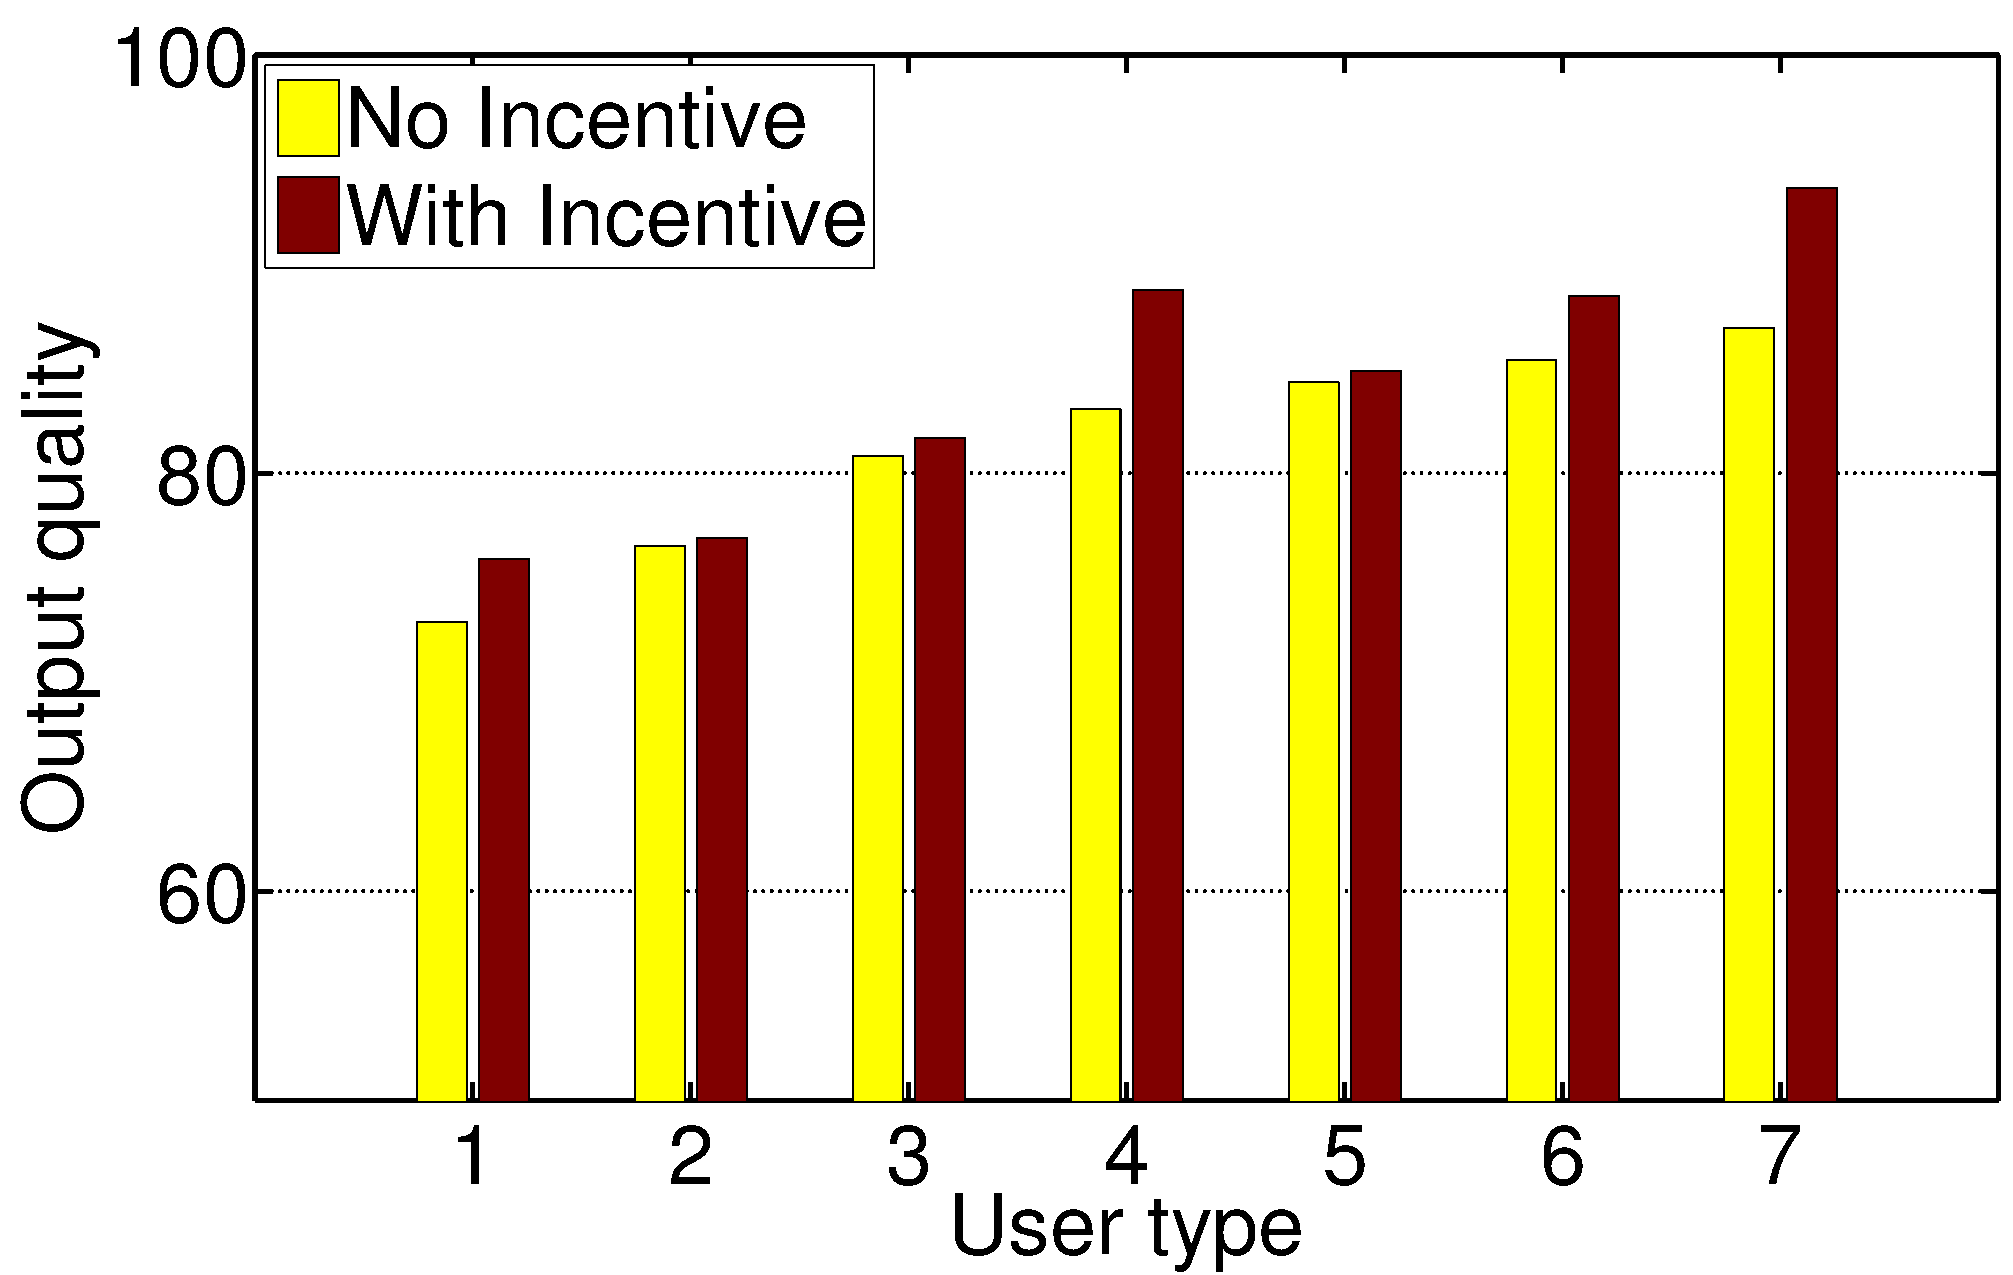
\includegraphics[width=\linewidth]{fig1}
	\caption{The figure with long long long long long long long long long long long long long long long long long long long long long long long long long long long long long long long long caption and links. (\url{https://goo.gl/VLCRBB}).}
\end{figure}



\lipsum[1-2]
\begin{landscape} % Require pdflscape and everypage packadge
	\begin{figure}[h]
		\centering
		% will generate blank page if use full  \linewidth
		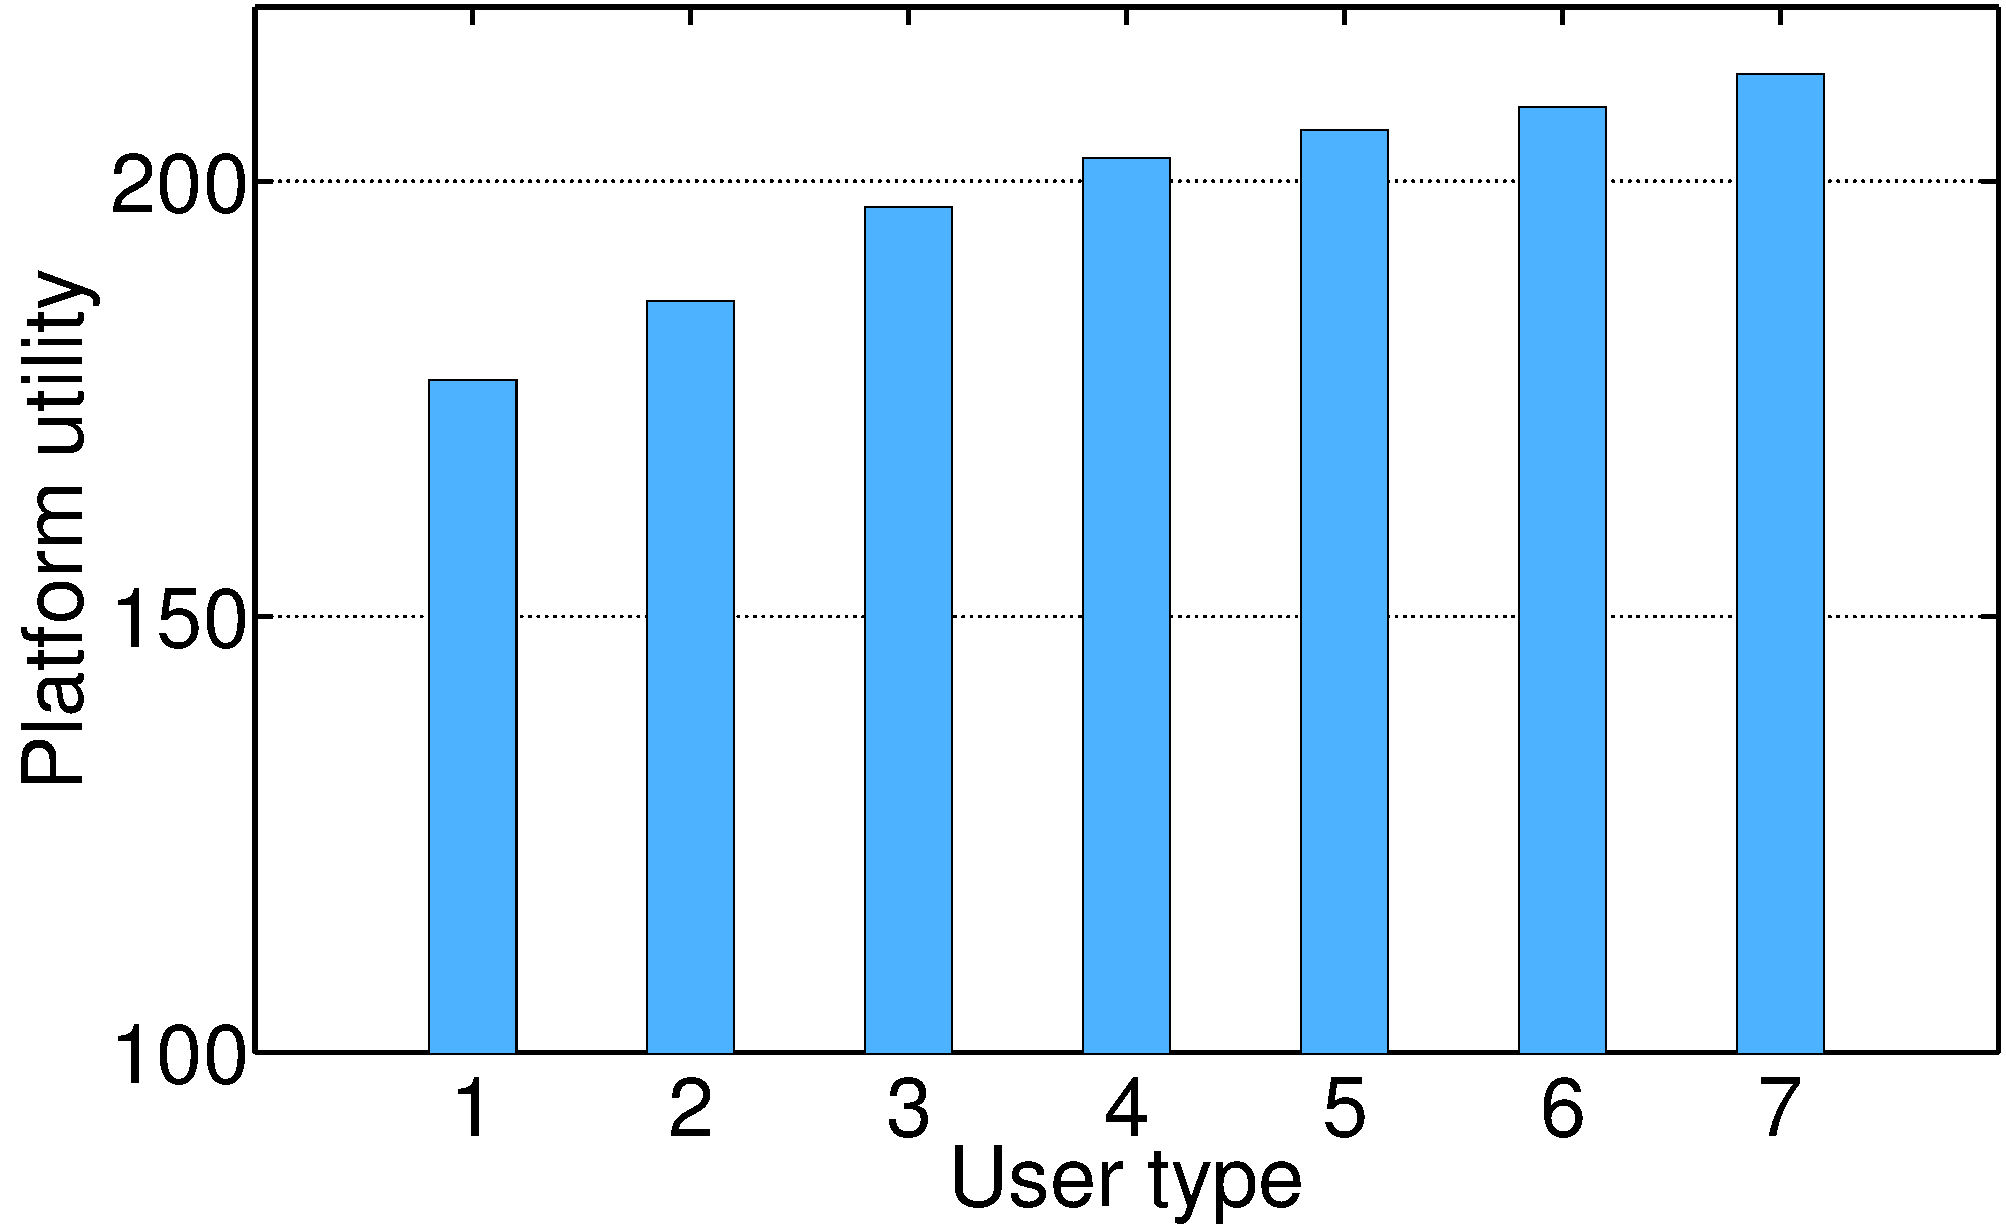
\includegraphics[width=.9\linewidth]{fig3} 
		\caption{Continues figures in landscape mode. (first)}
	\end{figure}

	\begin{figure}[h]
	\centering
	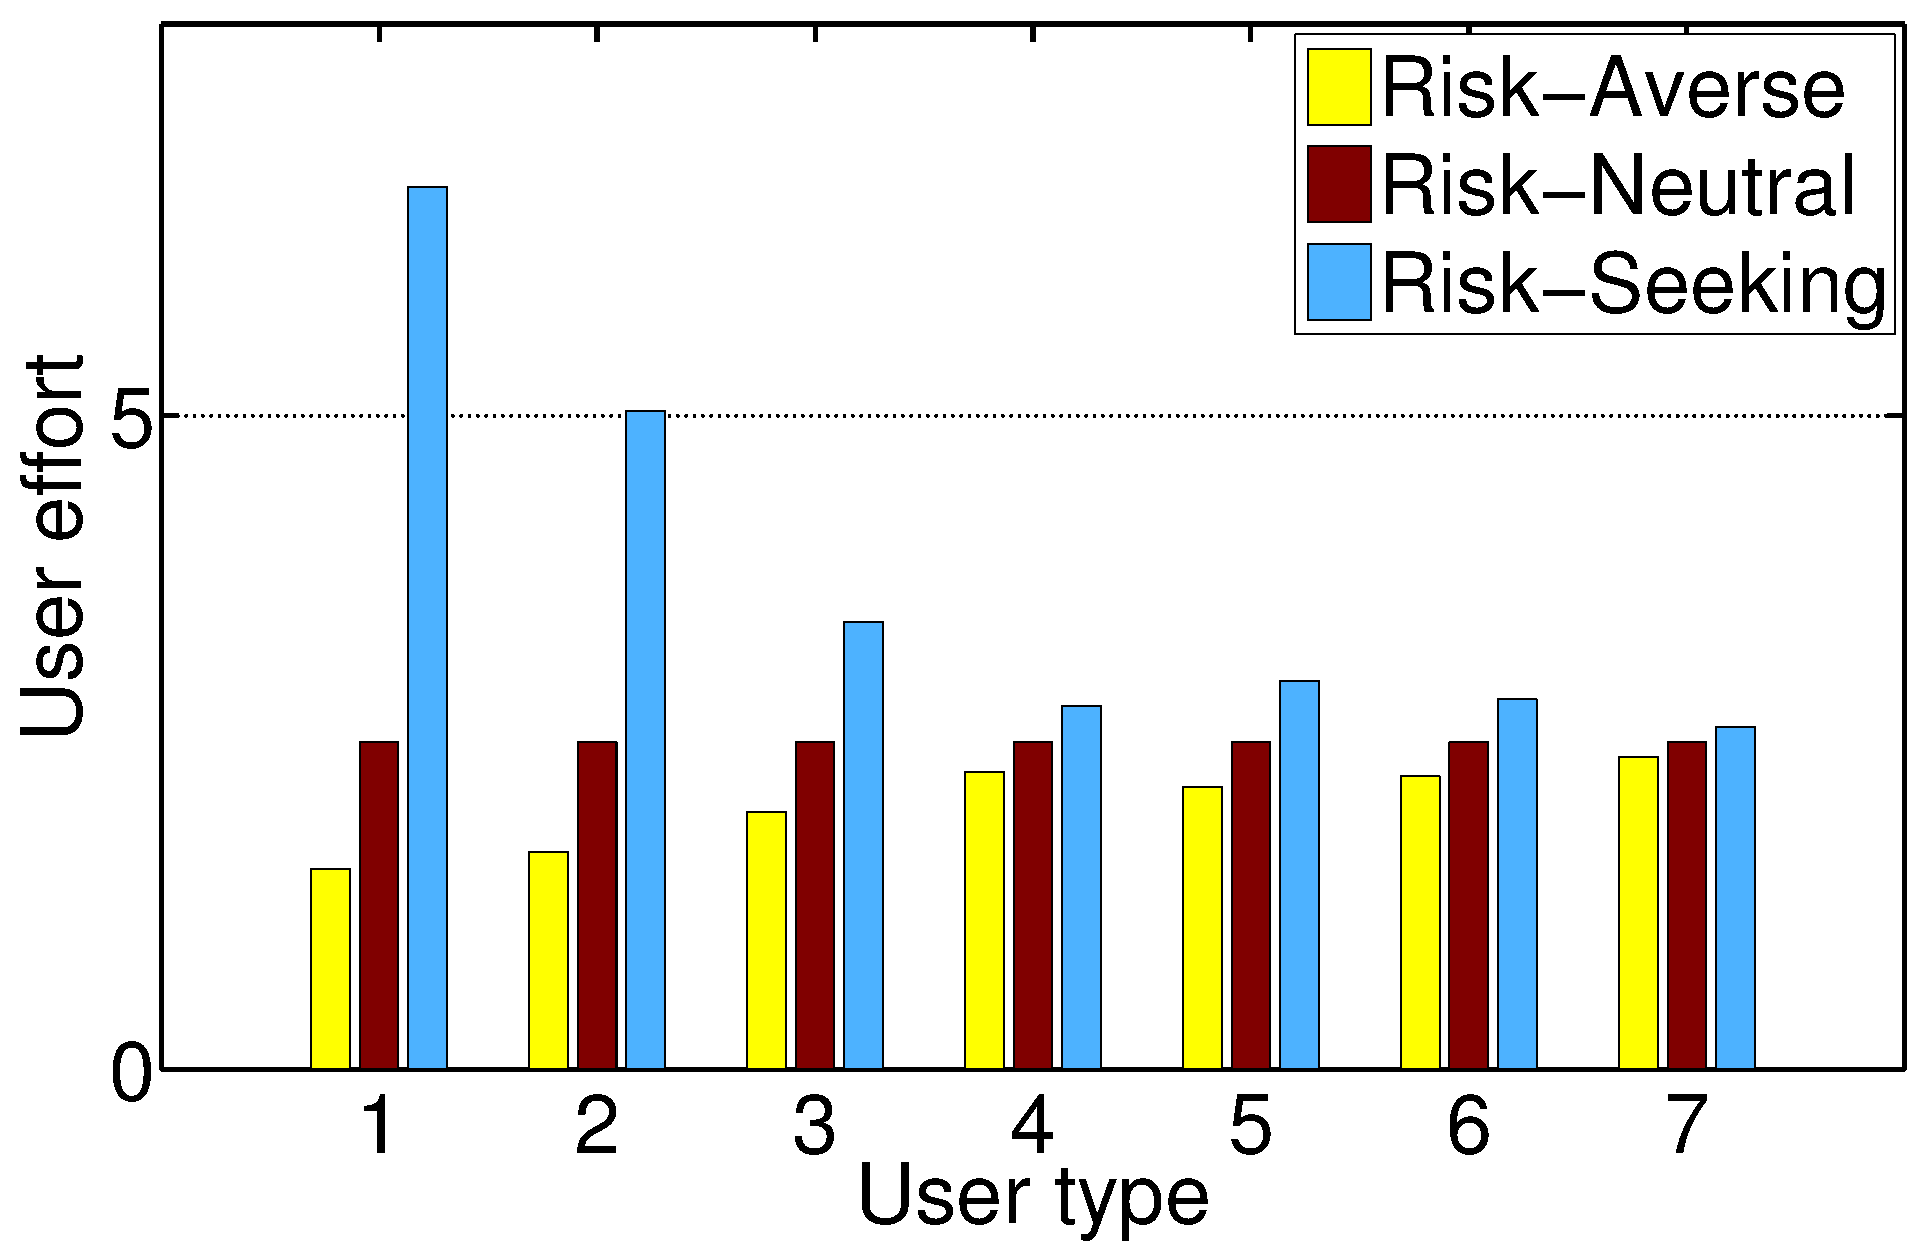
\includegraphics[width=\linewidth]{fig4}
	\caption{Continues figures in landscape mode. (second)}
	\end{figure}
\end{landscape}

Your figures should contain a caption which describes the figure to
the reader. Figure captions go below the figure. Your figures should
{\bfseries also} include a description suitable for screen readers, to
assist the visually-challenged to better understand your work.

Figure captions are placed {\itshape below} the figure.


\begin{landscape} % Require pdflscape and everypage packadge
	\begin{figure}[h]
		\centering
		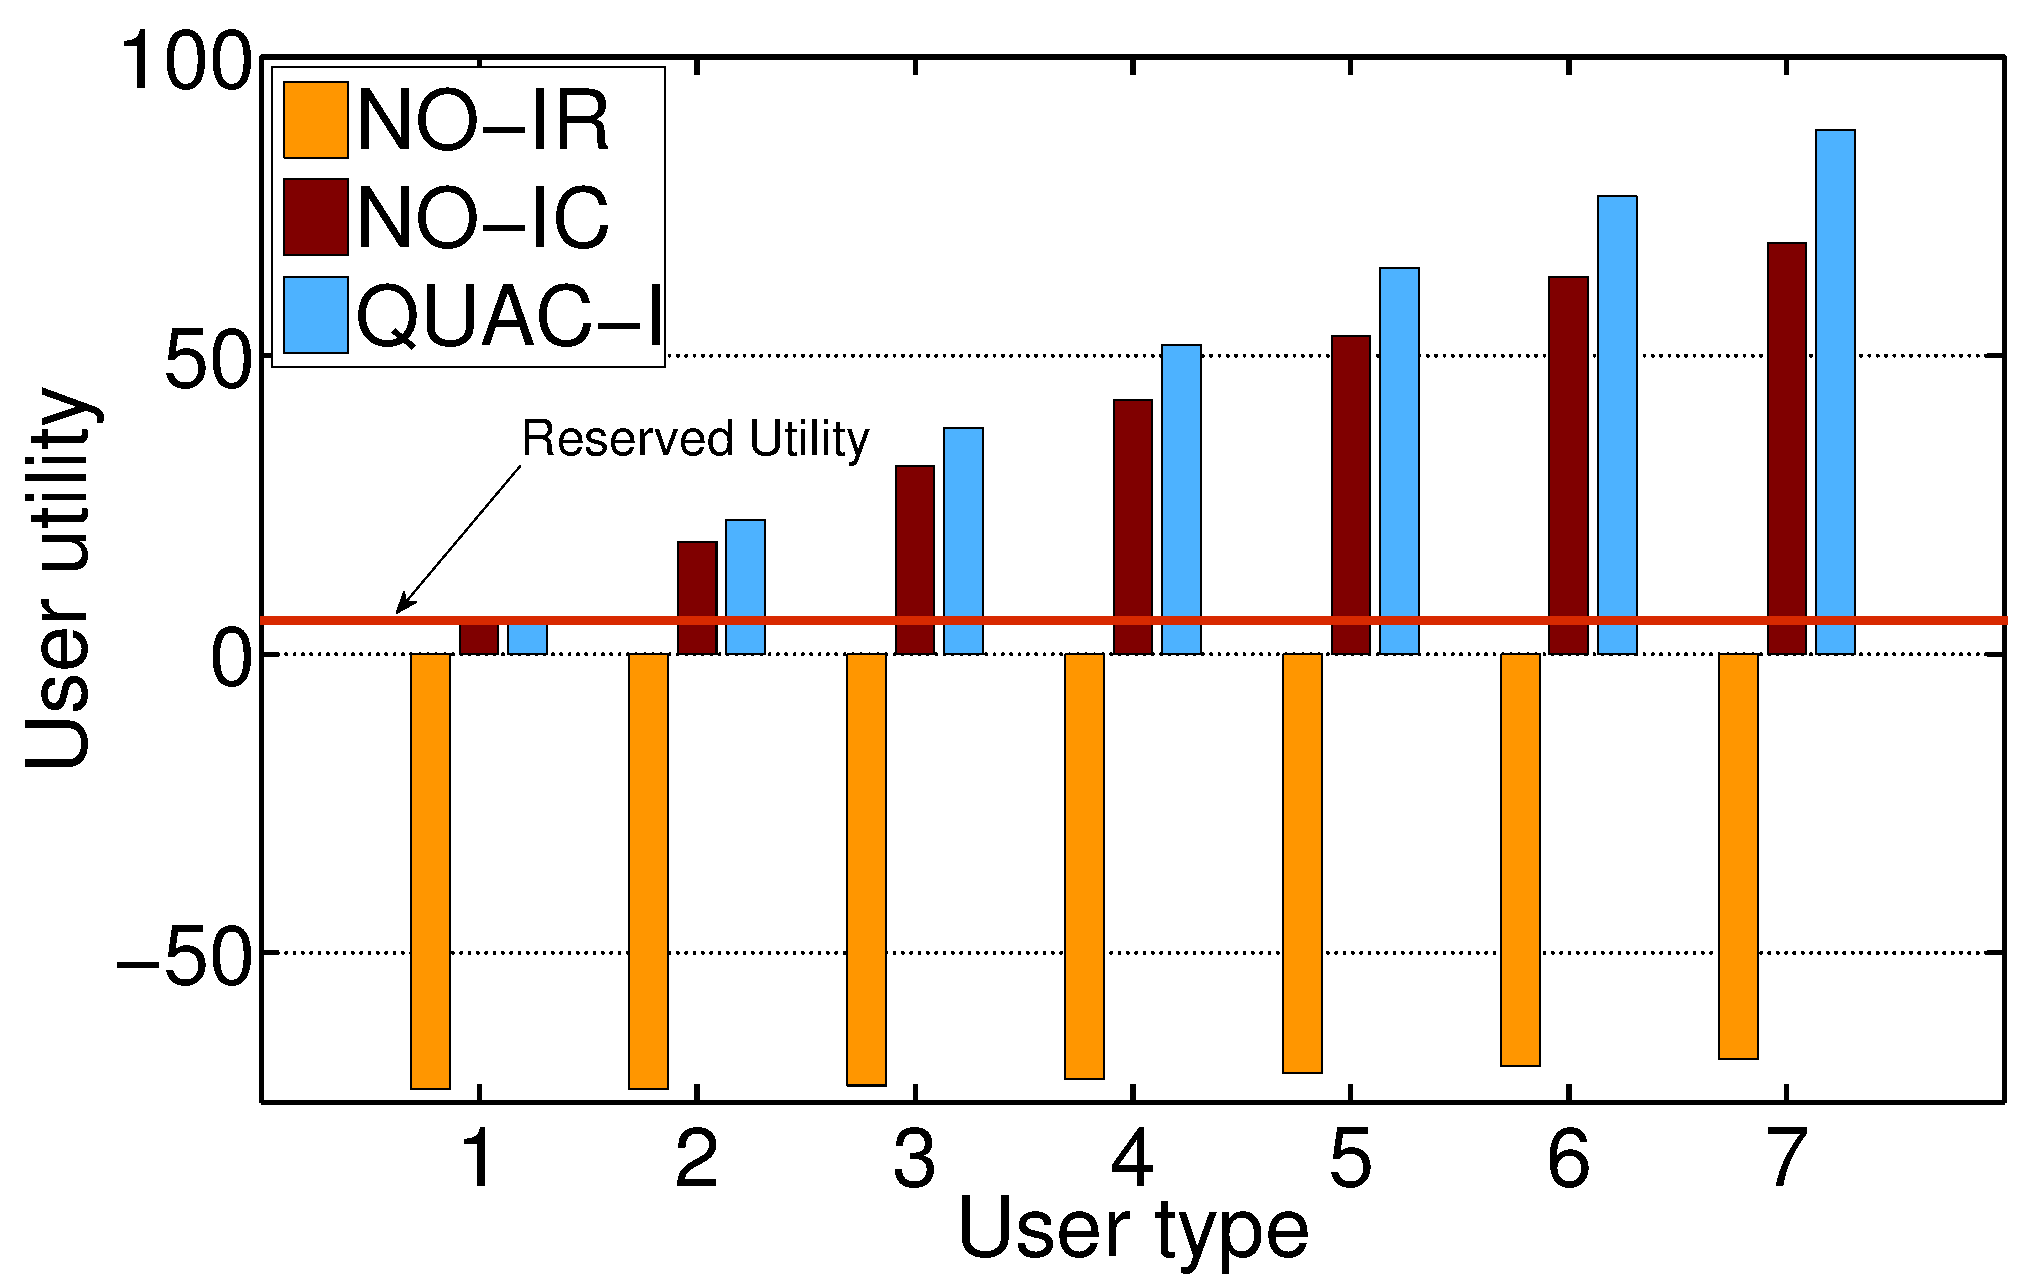
\includegraphics[width=.9\linewidth]{fig6}
		\caption{Example of a figure in landscape mode. Use \texttt{$\backslash$centering} to center the image}
	\end{figure}
\end{landscape}



\begin{figure}[h]
	\centering
	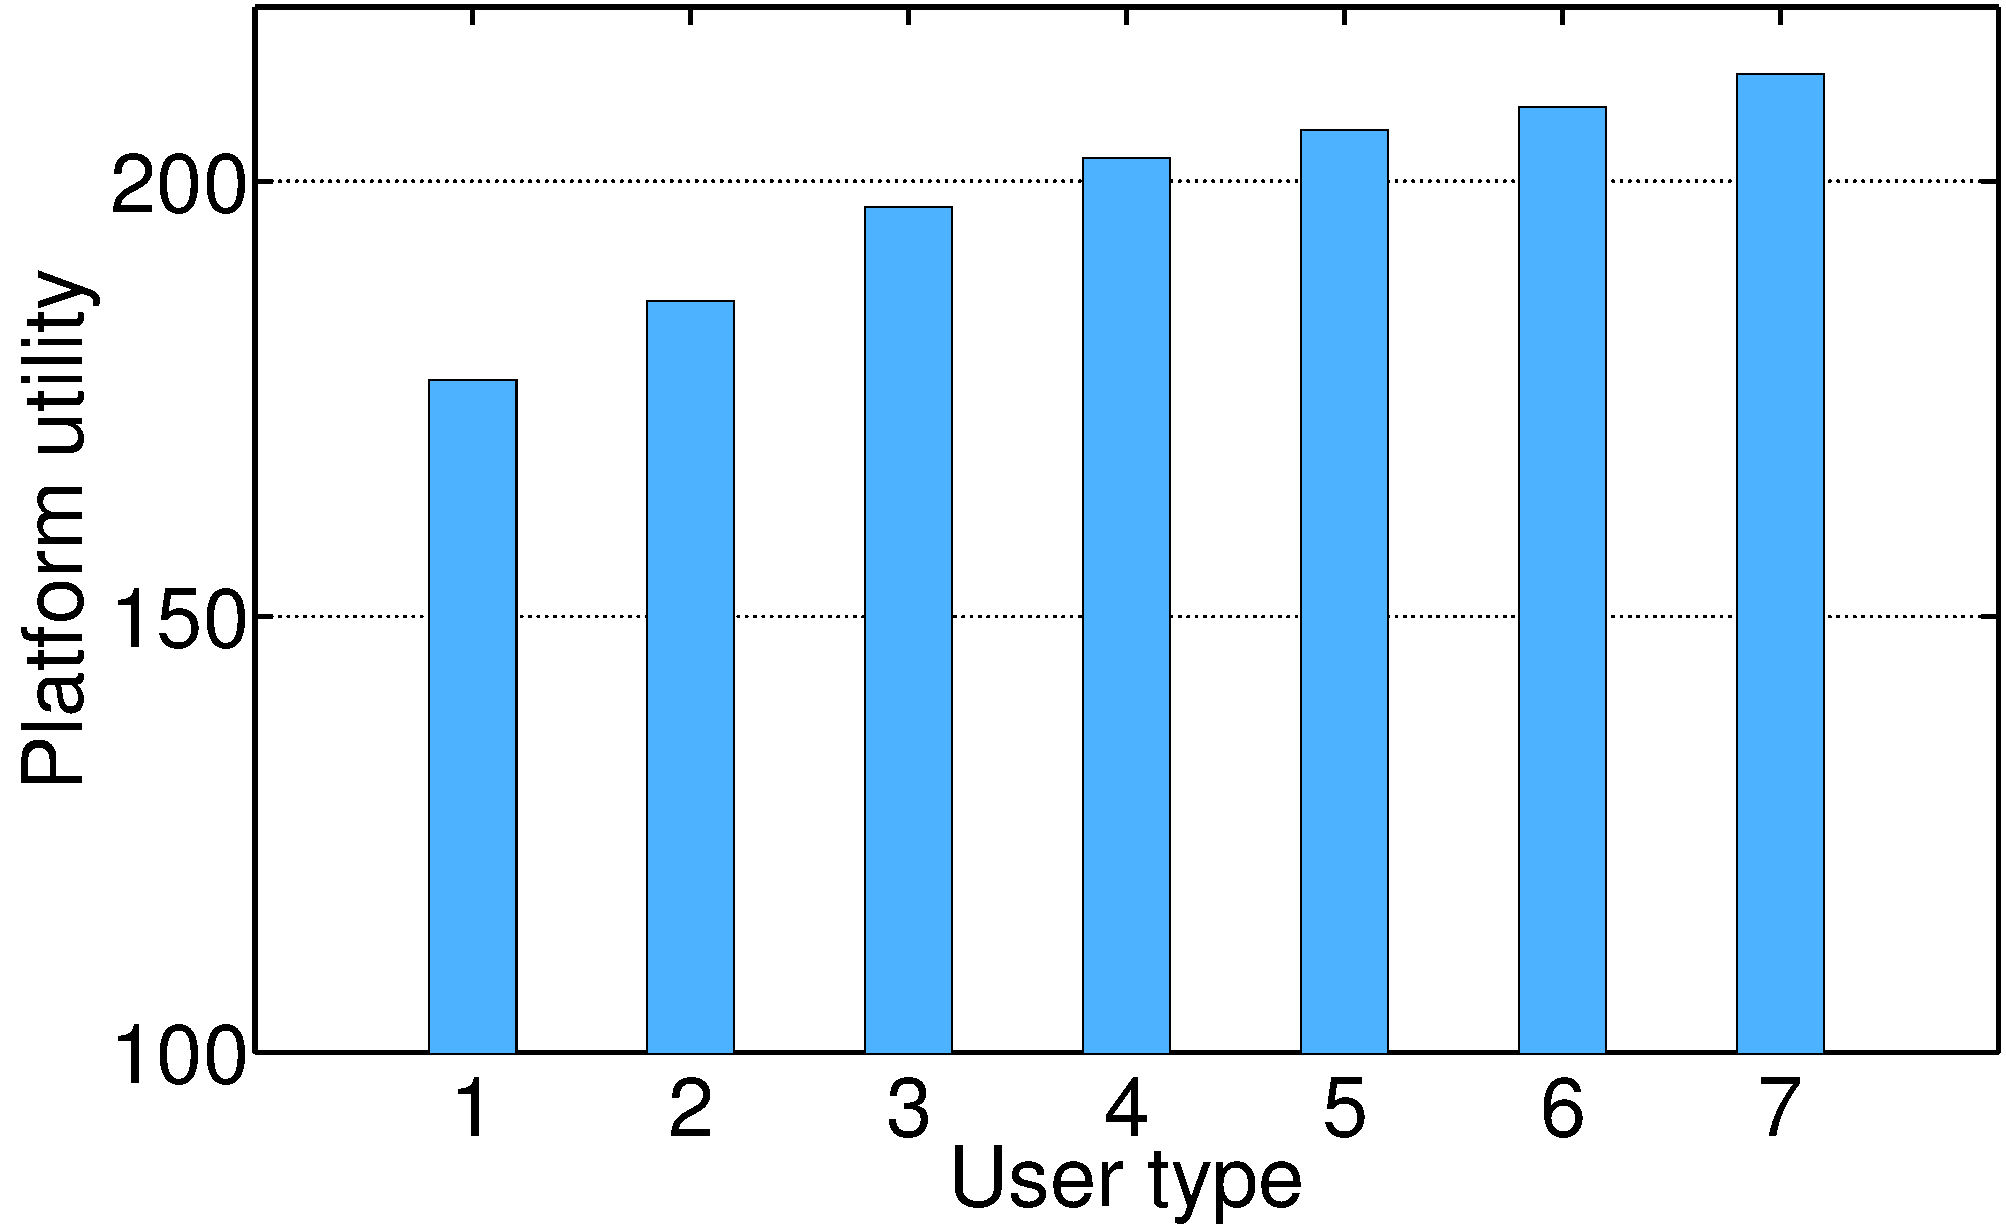
\includegraphics[width=\linewidth]{fig3}
	\caption[Short version caption for LoF, the original caption is really long]{The original realy long long long long long long long long long long long long long long long long long long long long long long long long long long long long long long figure caption.}
\end{figure}
%========================================
%              Section               
%======================================== 
\section{Tables}

The ``\verb|minesthesis|'' document class includes the ``\verb|booktabs|''
package --- \url{https://ctan.org/pkg/booktabs} --- for preparing
high-quality tables.

Table captions are placed {\itshape above} the table.

Because tables cannot be split across pages, the best placement for
them is typically the top of the page nearest their initial cite. To
ensure this proper ``floating'' placement of tables, use the
environment \textbf{table} to enclose the table's contents and the
table caption. The contents of the table itself must go in the
\textbf{tabular} environment, to be aligned properly in rows and
columns, with the desired horizontal and vertical rules. Again,
detailed instructions on \textbf{tabular} material are found in the
\textit{\LaTeX\ User's Guide}.

Immediately following this sentence is the point at which
Table~\ref{tab:freq} is included in the input file; compare the
placement of the table here with the table in the printed output of
this document.

\begin{table}[h]
	\caption{Frequency of Special Characters}
	\label{tab:freq}
	\centering
	\begin{tabular}{ccl}
		\toprule
		Non-English or Math & Frequency   & Comments          \\
		\midrule
		\O                  & 1 in 1,000  & For Swedish names \\
		$\pi$               & 1 in 5      & Common in math    \\
		\$                  & 4 in 5      & Used in business  \\
		$\Psi^2_1$          & 1 in 40,000 & Unexplained usage \\
		\bottomrule
	\end{tabular}
\end{table}


\begin{table*}[h]
	\caption{Some Typical Commands}
	\label{tab:commands}
	\centering
	\begin{tabular}{cclccr}
		\toprule
		Command                    & A Number & Comments         & Command                    & A Number & Comments         \\
		\midrule
		\texttt{{\char'134}author} & 100      & Author           & \texttt{{\char'134}author} & 100      & Author           \\
		\texttt{{\char'134}table}  & 300      & For tables       & \texttt{{\char'134}table}  & 300      & For tables       \\
		\texttt{{\char'134}table*} & 400      & For wider tables & \texttt{{\char'134}table*} & 400      & For wider tables \\
		\bottomrule
	\end{tabular}
\end{table*}

\begin{table*}[h]
	\caption{Some Typical Commands with borders}
	\label{tab:commandswithborders}
	\centering
	\begin{tabular}{|ccl|ccr|} % use | to add vertical lines
		\hline % use hline instead of toprule/midrule/bottomrule
		Command                    & A Number & Comments         & Command                    & A Number & Comments         \\
		\hline
		\texttt{{\char'134}author} & 100      & Author           & \texttt{{\char'134}author} & 100      & Author           \\
		\texttt{{\char'134}table}  & 300      & For tables       & \texttt{{\char'134}table}  & 300      & For tables       \\
		\texttt{{\char'134}table*} & 400      & For wider tables & \texttt{{\char'134}table*} & 400      & For wider tables \\
		\hline
	\end{tabular}
\end{table*}

To set a wider table, which takes up the whole width of the page's
live area, use the environment \textbf{table*} to enclose the table's
contents and the table caption. As with a single-column table, this
wide table will ``float'' to a location deemed more
desirable. Immediately following this sentence is the point at which
Table~\ref{tab:commands} is included in the input file; again, it is
instructive to compare the placement of the table here with the table
in the printed output of this document.
\begin{table}[h]
	\caption{Some table with really long long long long long long long long long long long long long long long long long long long long long long long long long long long long long long long long long long long caption}
	\label{tab:commandsnostar}
	\centering
	\begin{tabular}{cclccr}
		\toprule
		Command                    & A Number & Comments         & Command                    & A Number & Comments         \\
		\midrule
		\texttt{{\char'134}author} & 100      & Author           & \texttt{{\char'134}author} & 100      & Author           \\
		\texttt{{\char'134}table}  & 300      & For tables       & \texttt{{\char'134}table}  & 300      & For tables       \\
		\texttt{{\char'134}table*} & 400      & For wider tables & \texttt{{\char'134}table*} & 400      & For wider tables \\
		\bottomrule
	\end{tabular}
\end{table}



\begin{landscape}
	\begin{table}[h]
		\caption{A table in landscape mode}
		\label{tab:landscape}
%		\centering
		\begin{tabular}{cclccrlcr}
			\toprule
			Command                    & A Number & Comments         & Command                    & A Number & Comments         & Command                    & A Number & Comments         \\
			\midrule
			\texttt{{\char'134}author} & 100      & Author           & \texttt{{\char'134}author} & 100      & Author           & \texttt{{\char'134}author} & 100      & Author           \\
			\texttt{{\char'134}table}  & 300      & For tables       & \texttt{{\char'134}table}  & 300      & For tables       & \texttt{{\char'134}table}  & 300      & For tables       \\
			\texttt{{\char'134}table*} & 400      & For wider tables & \texttt{{\char'134}table*} & 400      & For wider tables & \texttt{{\char'134}table*} & 400      & For wider tables \\
			\texttt{{\char'134}author} & 100      & Author           & \texttt{{\char'134}author} & 100      & Author           & \texttt{{\char'134}author} & 100      & Author           \\
			\texttt{{\char'134}table}  & 300      & For tables       & \texttt{{\char'134}table}  & 300      & For tables       & \texttt{{\char'134}table}  & 300      & For tables       \\
			\texttt{{\char'134}table*} & 400      & For wider tables & \texttt{{\char'134}table*} & 400      & For wider tables & \texttt{{\char'134}table*} & 400      & For wider tables \\
			\texttt{{\char'134}author} & 100      & Author           & \texttt{{\char'134}author} & 100      & Author           & \texttt{{\char'134}author} & 100      & Author           \\
			\texttt{{\char'134}table}  & 300      & For tables       & \texttt{{\char'134}table}  & 300      & For tables       & \texttt{{\char'134}table}  & 300      & For tables       \\
			\texttt{{\char'134}table*} & 400      & For wider tables & \texttt{{\char'134}table*} & 400      & For wider tables & \texttt{{\char'134}table*} & 400      & For wider tables \\
			\texttt{{\char'134}author} & 100      & Author           & \texttt{{\char'134}author} & 100      & Author           & \texttt{{\char'134}author} & 100      & Author           \\
			\texttt{{\char'134}table}  & 300      & For tables       & \texttt{{\char'134}table}  & 300      & For tables       & \texttt{{\char'134}table}  & 300      & For tables       \\
			\texttt{{\char'134}table*} & 400      & For wider tables & \texttt{{\char'134}table*} & 400      & For wider tables & \texttt{{\char'134}table*} & 400      & For wider tables \\
			\bottomrule
		\end{tabular}
	\end{table}
\end{landscape}



%========================================
%              Section               
%======================================== 
\section{Section of Long Tables}
\lipsum[6-7]


\subsection{Currently supported publications}
\label{sec:pubs}


 \begin{longtable}{>{\ttfamily}p{0.2\textwidth}@{}p{0.8\textwidth}}
   \caption{ACM publications and arguments of the \cs{acmJournal}
   command Source: \url{https://www.acm.org/binaries/content/assets/publications/consolidated-tex-template/acmart.pdf}}
   \label{tab:pubs}\\
     \toprule
     \normalfont Abbreviation & Publication \\
     \midrule
 \endfirsthead
   \caption[]{ACM publications and arguments of the \cs{acmJournal}
   command (continued)}\\
     \toprule
     \normalfont Abbreviation & Publication \\
     \midrule
 \endhead
 \bottomrule
 \endfoot
CIE & ACM Computers in Entertainment \\
CSUR & ACM Computing Surveys\\
DGOV & Digital Government: Research and Practice \\
DTRAP &  Digital Threats: Research and Practice\\
HEALTH & ACM Transactions on Computing for Healthcare\\
IMWUT & PACM on Interactive, Mobile, Wearable and Ubiquitous
Technologies\\
JACM &  Journal of the ACM \\
JDIQ & ACM Journal of Data and Information Quality \\
JEA & ACM Journal of Experimental Algorithmics \\
JERIC & ACM Journal of Educational Resources in Computing\\
JETC & ACM Journal on Emerging Technologies in Computing Systems \\
JOCCH & ACM Journal on Computing and Cultural Heritage \\
PACMCGIT & Proceedings of the ACM on Computer Graphics and
Interactive Techniques\\
PACMHCI & PACM on Human-Computer Interaction\\
PACMPL & PACM on Programming Languages \\
POMACS & PACM on Measurement and Analysis of Computing Systems \\
TAAS & ACM Transactions on Autonomous and Adaptive Systems\\
TACCESS & ACM Transactions on Accessible Computing\\
TACO & ACM Transactions on Architecture and Code Optimization \\
TALG & ACM Transactions on Algorithms \\
TALLIP & ACM Transactions on Asian and Low-Resource Language
Information Processing\\
TAP & ACM Transactions on Applied Perception \\
TCPS & ACM Transactions on Cyber-Physical Systems\\
TDS & ACM Transactions on Data Science\\
TEAC & ACM Transactions on Economics and Computation\\
TECS & ACM Transactions on Embedded Computing Systems \\
TELO & ACM Transactions on Evolutionary Learning \\
THRI & ACM Transactions on Human-Robot Interaction\\
TIIS & ACM Transactions on Interactive Intelligent Systems\\
TIOT & ACM Transactions on Internet of Things \\
TISSEC & ACM Transactions on Information and System Security\\
TIST & ACM Transactions on Intelligent Systems and Technology \\
TKDD & ACM Transactions on Knowledge Discovery from Data\\
TMIS & ACM Transactions on Management Information Systems\\
TOCE & ACM Transactions on Computing Education\\
TOCHI & ACM Transactions on Computer-Human Interaction\\
TOCL & ACM Transactions on Computational Logic\\
TOCS & ACM Transactions on Computer Systems \\
TOCT & ACM Transactions on Computation Theory \\
TODAES & ACM Transactions on Design Automation of Electronic Systems\\
TODS & ACM Transactions on Database Systems\\
TOG & ACM Transactions on Graphics\\
TOIS & ACM Transactions on Information Systems\\
 \end{longtable}

\lipsum[3-4]

\begin{SingleSpace}
	\begin{longtable}{ccl}
		\caption[Feasible triples for a highly variable Grid]{Feasible triples for 
			highly variable Grid, MLMMH. source:\url{http://users.sdsc.edu/~ssmallen/latex/longtable.html}} \label{grid_mlmmh} \\
		
		\toprule
		Times(s) & Triple chosen & Other feasible triples \\
		\midrule
		\endfirsthead
		
		\tablename~\thetable{}~Continued\\
		\toprule
		Times(s) & Triple chosen & Other feasible triples \\
		\midrule
		\endhead
		\bottomrule		
		\endfoot
		\endlastfoot
		
		0 & (1, 11, 13725) & (1, 12, 10980), (1, 13, 8235), (2, 2, 0), (3, 1, 0) \\
		2745 & (1, 12, 10980) & (1, 13, 8235), (2, 2, 0), (2, 3, 0), (3, 1, 0) \\
		5490 & (1, 12, 13725) & (2, 2, 2745), (2, 3, 0), (3, 1, 0) \\
		8235 & (1, 12, 16470) & (1, 13, 13725), (2, 2, 2745), (2, 3, 0), (3, 1, 0) \\
		10980 & (1, 12, 16470) & (1, 13, 13725), (2, 2, 2745), (2, 3, 0), (3, 1, 0) \\
		13725 & (1, 12, 16470) & (1, 13, 13725), (2, 2, 2745), (2, 3, 0), (3, 1, 0) \\
		16470 & (1, 13, 16470) & (2, 2, 2745), (2, 3, 0), (3, 1, 0) \\
		19215 & (1, 12, 16470) & (1, 13, 13725), (2, 2, 2745), (2, 3, 0), (3, 1, 0) \\
		21960 & (1, 12, 16470) & (1, 13, 13725), (2, 2, 2745), (2, 3, 0), (3, 1, 0) \\
		24705 & (1, 12, 16470) & (1, 13, 13725), (2, 2, 2745), (2, 3, 0), (3, 1, 0) \\
		27450 & (1, 12, 16470) & (1, 13, 13725), (2, 2, 2745), (2, 3, 0), (3, 1, 0) \\
		30195 & (2, 2, 2745) & (2, 3, 0), (3, 1, 0) \\
		32940 & (1, 13, 16470) & (2, 2, 2745), (2, 3, 0), (3, 1, 0) \\
		35685 & (1, 13, 13725) & (2, 2, 2745), (2, 3, 0), (3, 1, 0) \\
		38430 & (1, 13, 10980) & (2, 2, 2745), (2, 3, 0), (3, 1, 0) \\
		41175 & (1, 12, 13725) & (1, 13, 10980), (2, 2, 2745), (2, 3, 0), (3, 1, 0) \\
		43920 & (1, 13, 10980) & (2, 2, 2745), (2, 3, 0), (3, 1, 0) \\
		46665 & (2, 2, 2745) & (2, 3, 0), (3, 1, 0) \\
		49410 & (2, 2, 2745) & (2, 3, 0), (3, 1, 0) \\
		52155 & (1, 12, 16470) & (1, 13, 13725), (2, 2, 2745), (2, 3, 0), (3, 1, 0) \\
		54900 & (1, 13, 13725) & (2, 2, 2745), (2, 3, 0), (3, 1, 0) \\
		57645 & (1, 13, 13725) & (2, 2, 2745), (2, 3, 0), (3, 1, 0) \\
		60390 & (1, 12, 13725) & (2, 2, 2745), (2, 3, 0), (3, 1, 0) \\
		63135 & (1, 13, 16470) & (2, 2, 2745), (2, 3, 0), (3, 1, 0) \\
		65880 & (1, 13, 16470) & (2, 2, 2745), (2, 3, 0), (3, 1, 0) \\
		68625 & (2, 2, 2745) & (2, 3, 0), (3, 1, 0) \\
		71370 & (1, 13, 13725) & (2, 2, 2745), (2, 3, 0), (3, 1, 0) \\
		74115 & (1, 12, 13725) & (2, 2, 2745), (2, 3, 0), (3, 1, 0) \\
		76860 & (1, 13, 13725) & (2, 2, 2745), (2, 3, 0), (3, 1, 0) \\
		79605 & (1, 13, 13725) & (2, 2, 2745), (2, 3, 0), (3, 1, 0) \\
		82350 & (1, 12, 13725) & (2, 2, 2745), (2, 3, 0), (3, 1, 0) \\
		85095 & (1, 12, 13725) & (1, 13, 10980), (2, 2, 2745), (2, 3, 0), (3, 1, 0) \\
		87840 & (1, 13, 16470) & (2, 2, 2745), (2, 3, 0), (3, 1, 0) \\
		90585 & (1, 13, 16470) & (2, 2, 2745), (2, 3, 0), (3, 1, 0) \\
		93330 & (1, 13, 13725) & (2, 2, 2745), (2, 3, 0), (3, 1, 0) \\
		96075 & (1, 13, 16470) & (2, 2, 2745), (2, 3, 0), (3, 1, 0) \\
		98820 & (1, 13, 16470) & (2, 2, 2745), (2, 3, 0), (3, 1, 0) \\
		101565 & (1, 13, 13725) & (2, 2, 2745), (2, 3, 0), (3, 1, 0) \\
		104310 & (1, 13, 16470) & (2, 2, 2745), (2, 3, 0), (3, 1, 0) \\
		107055 & (1, 13, 13725) & (2, 2, 2745), (2, 3, 0), (3, 1, 0) \\
		109800 & (1, 13, 13725) & (2, 2, 2745), (2, 3, 0), (3, 1, 0) \\
		112545 & (1, 12, 16470) & (1, 13, 13725), (2, 2, 2745), (2, 3, 0), (3, 1, 0) \\
		115290 & (1, 13, 16470) & (2, 2, 2745), (2, 3, 0), (3, 1, 0) \\
		118035 & (1, 13, 13725) & (2, 2, 2745), (2, 3, 0), (3, 1, 0) \\
		120780 & (1, 13, 16470) & (2, 2, 2745), (2, 3, 0), (3, 1, 0) \\
		123525 & (1, 13, 13725) & (2, 2, 2745), (2, 3, 0), (3, 1, 0) \\
		126270 & (1, 12, 16470) & (1, 13, 13725), (2, 2, 2745), (2, 3, 0), (3, 1, 0) \\
		129015 & (2, 2, 2745) & (2, 3, 0), (3, 1, 0) \\
		131760 & (2, 2, 2745) & (2, 3, 0), (3, 1, 0) \\
		134505 & (1, 13, 16470) & (2, 2, 2745), (2, 3, 0), (3, 1, 0) \\
		137250 & (1, 13, 13725) & (2, 2, 2745), (2, 3, 0), (3, 1, 0) \\
		139995 & (2, 2, 2745) & (2, 3, 0), (3, 1, 0) \\
		142740 & (2, 2, 2745) & (2, 3, 0), (3, 1, 0) \\
		145485 & (1, 12, 16470) & (1, 13, 13725), (2, 2, 2745), (2, 3, 0), (3, 1, 0) \\
		148230 & (2, 2, 2745) & (2, 3, 0), (3, 1, 0) \\
		150975 & (1, 13, 16470) & (2, 2, 2745), (2, 3, 0), (3, 1, 0) \\
		153720 & (1, 12, 13725) & (2, 2, 2745), (2, 3, 0), (3, 1, 0) \\
		156465 & (1, 13, 13725) & (2, 2, 2745), (2, 3, 0), (3, 1, 0) \\
		159210 & (1, 13, 13725) & (2, 2, 2745), (2, 3, 0), (3, 1, 0) \\
		161955 & (1, 13, 16470) & (2, 2, 2745), (2, 3, 0), (3, 1, 0) \\
		164700 & (1, 13, 13725) & (2, 2, 2745), (2, 3, 0), (3, 1, 0) \\
		\bottomrule
	\end{longtable}
\end{SingleSpace}

\lipsum[3-4]